%\documentclass{vgtc}
% commented
%\usepackage{amsmath, url, graphicx, algorithm, ctable, times}
%\usepackage{algpseudocode}
%\usepackage{enumitem}

% newly added per NIPS
%\documentclass{article} % For LaTeX2e
%\usepackage{hyperref}
%\usepackage{url}
%

\documentclass{article}
\usepackage{fullpage,enumitem,amsmath,
amssymb,graphicx,url,listings,color,hyperref,floatrow,natbib,pdfpages}


%\definecolor{mygreen}{RGB}{28,172,0}  % color values Red, Green, Blue
%\definecolor{mylilas}{RGB}{170,55,241}

%\usepackage{nips13submit_e,times}

%\makeatletter
%\renewcommand{\ALG@beginalgorithmic}{\small}
%\makeatother

\usepackage[caption=false]{subfig}
%\marginsize{1.5cm}{1.5cm}{1cm}{1cm}
\captionsetup{font = scriptsize}
%\makesavenoteenv{tabular}


\begin{document}

\pagestyle{empty} 
%\title{Large AI Agent for Lunar Lander}

\title{\textbf{ AI Agent for Lunar Lander}}

\author{Prabhjot Singh Rai  (prabhjot) \\ 
\and Abhishek Bharani (abharani) \\
\and Amey Naik (ameynaik)
}


\maketitle

\section{Task Definition}
\label{intro}

The task accomplished by this project is to build an AI agent for the game of Lunar Lander defined by openAI gym in Box2D format. Here, a lunar lander needs to land with zero velocity between the flags on a landing pad as shown in the figure. with a constant high reward. This is accomplished by Reinforcement Learning, particularly by applying different Deep Q-learning techniques. This project has explored Full DQN\citep{DoubleQ-learning}, Double DQN\citep{DoubleQ-learning}, and Dueling DQN\citep{Dueling}, to solve the game. We consider the game as solved when the agent starts getting an average reward of 200 over 100 consecutive episodes. Moreover, the performance of different DQN variants are compared to solve the problem. \\


\begin{figure}[!ht]
%\begin{figure}%
%\vspace*{\fill}
\centering

\includegraphics[scale=0.50,width=0.50\columnwidth]{figures/game.png}%
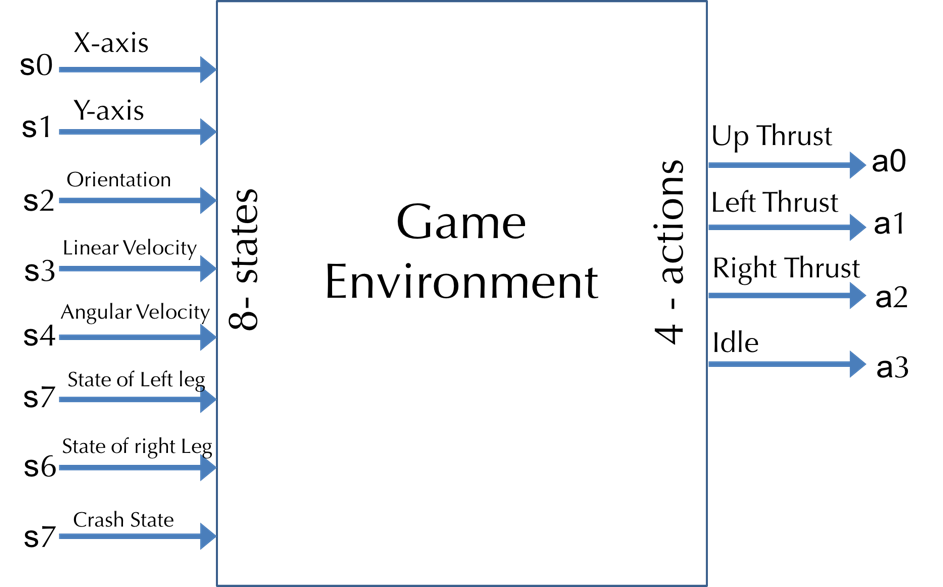
\includegraphics[scale=0.50,width=0.50\columnwidth]{figures/game_env.png}%
\caption{ Lunar Lander and Game Environment }%
\label{fig:Visualization}%
\end{figure}
%\vfill}

Since, the problem involves high dimensional and continuous state
space, standard Q-learning cannot solve this problem unless some amount of discretization is done. Due to this difficulty, Deep Q-Network (DQN) was the choice. 





\section{Infrastructure}
\label{sec:rel}
We have used OpenAI gym library to train our agent. Although some insights are provided in Box2D Lunar Lander on OpenAI website, but thorough exploration of actions, state space, environment etc. were done before starting to solve the problem. Following is the description:

\subsection{Actions}
In this game, four discrete actions are available to the playing agent at any time frame: 

\begin{enumerate}[label=(\alph*)]
\item Do nothing
\item Fire left orientation engine (rotates the lunar lander clockwise)
\item Fire main engine (provides upward thrust)
\item Fire right orientation engine (rotates the lunar lander anti-clockwise)
\end{enumerate}

The agent can choose only one action among the given actions at a given time frame.

\subsection{Terrain} 
The terrain is a combination of 10 points, and the helipad(landing zone) is fixed between 5th and 6th points towards the center. The values of the height of the landing zone(5th and 6th points on the terrain) are viewport height divided by 4, and the rest of the points are randomly sampled between 0 to H/2 using \textit{numpy} random and smoothened (averaging 3 continuous points).

\subsection{Initial State}

The state is 8 dimensional values of different parameters of the lunar lander at any given time. The starting state is randomly initialized (the lunar lander takes a step in the world through the "idle" action) with certain bounds based on the environment.

Inspecting code of open\_ai lunar lander, we see that the initial states are defined by simulating the environment in one frame (calling box world simulation using time step as $1/FPS$). Using this simulation, elaborating the initial state as follows:

\begin{enumerate}
\item Position X (Initial Position X: final x which changed from half of viewport width to a value after taking "idle" action before the simulation)
\item Position Y (Initial Position Y: final y which changed from from the viewport height to a value after taking "idle" action before simulation)
\item Velocity X (Initial Velocity X: final velocity x changed from 0 to a value after taking "idle" action before simulation)
\item Velocity Y (Initial Velocity Y: final velocity y which changed from 0 to a value after taking "idle" action before simulation)
\item Current lander angle (Initial lander angle: final lander angle after simulation on "idle" action from 0 degrees)
\item Angular velocity (Initial angular velocity: final angular velocity after simulation on "idle" action from 0 angular velocity)
\item Left leg contacted the surface (Initial value: False, since there's is no probability that the lunar lander's leg will touch the moon surface when at the top)
\item Right leg contacted the surface (Initial value: False)
\end{enumerate}

\subsection{End State}

The episode ends in the following scenarios:

\begin{enumerate}
\item  When the lunar lander goes outside of the viewport bounds, the game is over with -100 is negative reward.
\item  When the lunar lander touches the ground with a high velocity
\item When the lunar lander touches the ground with body part except the legs
\item When the lunar lander stabilises on the moon's surface (change in shape of lunar lander is constantly 0 for a number of frames)
\end{enumerate}

\subsection{Rewards and Transitions}

Before defining the rewards, let's define the shape of the lunar lander which decides the rewards. The shape of the lunar lander is a function of position coordinates $(x, y)$, linear velocities $(v_x, v_y)$, lander angle $\theta$ and contact of both the lander legs. We are interested in finding the change of shape at every step for the lunar lander to calculate the rewards for each given action. Shape change is given by subtraction of previous shape and current shape. Formally, shaping at time frame $t$:

\begin{align*}
\text{shaping}_{t} = &- 100*(x^2 + y^2) \\
           & - 100*(v_x^2 + v_y^2) \\
            &- 100*abs(\theta) + 10*(\text{Left leg contacted}) + 10*(\text{Right leg contacted}) \\
\text{shape change} = & \text{shaping}_t - \text{shaping}_{t-1}
\end{align*}

The rewards are defined as follows:

\begin{enumerate}
\item If the lunar lander crashes, or goes out of the bounds: $-100$
\item If the lunar lander is not awake anymore (stabilises at 0 shape change): $+100$
\item Doing nothing: shape change 
\item Firing the engine: shape change - 0.3
\item Rotating: shape change - 0.03
\end{enumerate}

The total reward will automatically be a sum of all the rewards at each time frame, and if the lander touches the ground with it's legs, will add those rewards to the total rewards earned during an episode. Transition probabilities are unknown, we get next states by simulating the lunar lander in the box environment given the current state and action taken. \\

\textbf{Note}: The transition probabilities and rewards are unknown to our agent, which it will try to figure out through exploration and incorporate in learning. 


\section{Models and different Approaches}

\subsection{DQN Introduction}

Model-free based Deep Q Network algorithm was chosen specifically for the state size and complexity. DQN builds off of Q-learning algorithms by using a Deep Neural Network (DNN) for approximating the state-action value function, Q(s, a). Function Q(s, a) is defined such that for given state $s$ and action $a$ it returns an estimate of a total reward we would achieve starting at this state, taking the action and then following some policy. Let’s call the Q function for the optimal policies $Q_{opt}$.
 $Q_{opt}$ with discounting can be written as 
 \begin{equation}
Q_{opt}(s,a) = r_{0} + \gamma r_{1} + \gamma^{2} r_{2} + ...
\end{equation}
Here, $r$ stands for rewards. $\gamma$ is called a discount factor and when set it to $\gamma < $  1 , it makes sure that the sum in the formula is finite. The $\gamma$ controls how much the function Q in state $s$ depends on the future and so it can be thought of as how much ahead the agent sees.  \newline
The above equation can be rewritten in a recursive form.
 \begin{equation}
Q_{opt}(s,a) = r_{0} + \gamma max_{a}Q_{opt}(s',a)
\end{equation}
This equation is proven to converge to the desired $Q_{opt}$, with finite number of states and each of the state-action pair is presented repeatedly. However, the Lunar Lander state space is real and continuous. We cannot store infinite number of values for every possible state. Instead, we  approximate the Q function with a neural network. This network will take a state as an input and produce an estimation of the Q function for each action. This network with multiple layers is called Deep Q-network (DQN).
\newline \newline
\textbf{Experience Replay} \newline \newline
During each simulation step, the agent perform an action $a$ in state $s$, receives immediate reward $r$ and come to a new state $s’$.
\newline
There are two problems with online learning - \newline
1. The samples arrive in order they are experienced and as such are highly correlated. This might cause overfitting.
\newline
2. Throwing away each sample immediately after we use it. This means we are not using our experience effectively.
\newline
The key idea of 'experience replay' is that we store these $(s, a, r, s')$ transitions in a memory and during each learning step, sample a random batch and perform a gradient descend on it. This way we solve both issues.
After reaching the finite allotted memory capacity, the oldest sample is discarded.
\newline \newline
\textbf{Exploration}
To find out that actions which might be better then others, we use $\epsilon$ greedy policy. This policy behaves greedily most of the time, but chooses a random action with probability $\epsilon$. $\epsilon$ will be a hyper-parameter played with to make sure our agent learns fast enough while consistently performing better.

\subsection{Full DQN}
In DQN algorithm we set targets for gradient descend as:
\begin{equation}
Q_{opt}(s,a) = r_{0} + \gamma max_{a}Q_{opt}(s',a)
\end{equation}
We see that the target depends on the current network. A neural network works as a whole, and so each update to a point in the Q function also influences whole area around that point. And the points of $Q(s, a)$ and $Q(s’, a)$ are very close together, because each sample describes a transition from $s$ to $s’$. This leads to a problem that with each update, the target is likely to shift. This can lead to instabilities, oscillations or divergence.
\newline
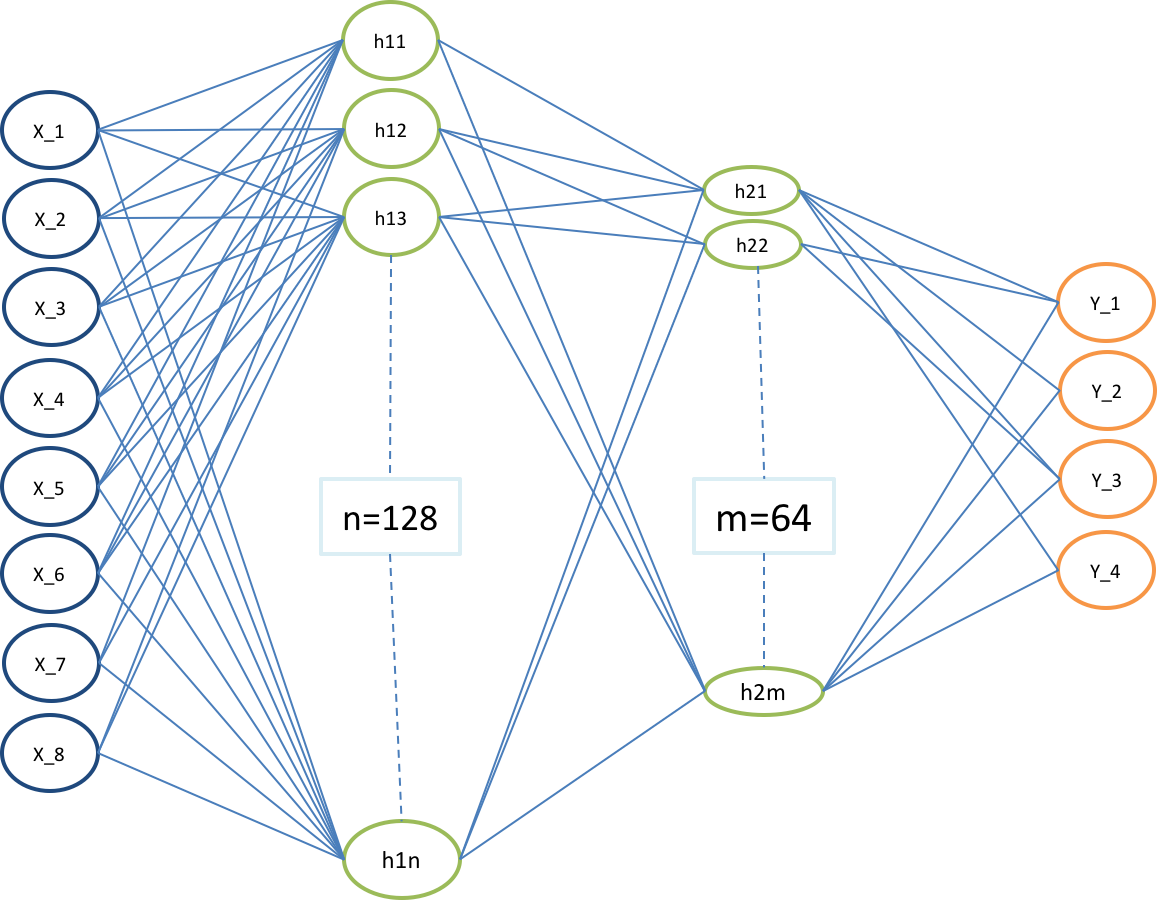
\includegraphics[scale=0.75,width=0.75\columnwidth]{figures/NN.png}%
\newline
To overcome this problem, researches proposed to use a separate target network for setting the targets. This network is a mere copy of the previous network, but frozen in time. It provides stable $\tilde{Q}$ values and allows the algorithm to converge to the specified target:
\begin{equation}
Q(s, a) \xrightarrow{} r + \gamma max_a \tilde{Q}(s', a)
\end{equation}

After several steps, the target network is updated, just by copying the weights from the current network. To be effective, the interval between updates has to be large enough to leave enough time for the original network to converge. \newline
For lunar lander, we update target model after every episode.

\subsection{Double DQN}
One problem in the DQN algorithm is that the agent tends to overestimate the Q function value, due to the max in the formula used to set targets.
Because of the max in the formula, the action with the highest positive/negative error could be selected and this value might subsequently propagate further to other states. This leads to bias – value overestimation. This severe impact on stability of the learning algorithm.
\newline
In this new algorithm, two Q functions $Q_{1}$ and $Q_2$ – are independently learned. One function is then used to determine the maximizing action and second to estimate its value. Either $Q_1$ or $Q_2$ is updated randomly with a formula:
\begin{equation}
Q_1(s, a) \xrightarrow{} r + \gamma Q_2(s', argmax_a Q_1(s', a)) 
\end{equation}
or
\begin{equation}
Q_2(s, a) \xrightarrow{} r + \gamma Q_1(s', argmax_a Q_2(s', a)) 
\end{equation}
It was proven that by decoupling the maximizing action from its value in this way, one can indeed eliminate the maximization bias.
\newline
When thinking about implementation into the DQN algorithm, we can leverage the fact that we already have two different networks giving us two different estimates Q and $\tilde{Q}$ (target network). Although not really independent, it allows us to change our algorithm in a really simple way.
\newline
The original target formula would change to:
\begin{equation}
Q(s, a) \xrightarrow{} r + \gamma \tilde{Q}(s', argmax_a Q(s', a))
\end{equation}
We could observe that Double DQN was more stable than Full DQN.
 
\subsection{Dueling layer DQN}
Q(s,a) represents the value of a given action $a$ chosen in state $s$, V(s) represents the value of the state independent of action. By definition, $V(s)=max_{a}Q(s,a)$. Thus, A(s,a) provides a relative measure of the utility of actions in s. The insight behind the dueling network architecture is that sometimes the exact choice of action does not matter so much, and so the state could be more explicitly modeled, independent of the action. There are two neural networks — one learns to provide an estimate of the value at every timestep, and the other calculates potential advantages of each action, and the two are combined for a single action-advantage Q function. We can achieve more robust estimates of state value by decoupling it from the necessity of being attached to specific actions.
 [FIXME https://arxiv.org/pdf/1511.06581.pdf]
\newline
\begin{equation}
Q(s,a) \rightarrow A(s,a) + V(s)
\end{equation}
The above equation is unidentifiable in the sense that given $Q$
we cannot recover $V$ and $A$ uniquely. This lack of identifiability is mirrored by poor practical performance when this equation is used directly. To address this issue of identifiability, we can force the advantage
function estimator to have zero advantage at the
chosen action. That is, we let the last module of the network
implement the forward mapping.
\begin{equation}
Q(s,a; \theta, \alpha, \beta) \rightarrow V(s; \theta, \beta) + (A(s,a\theta, \alpha) - max_{a' \epsilon |A|} A(s,a';\theta,\alpha ))
\end{equation}
An alternative module replaces the max operator with an
average. On the one hand this loses the original semantics of V and
A because they are now off-target by a constant, but on
the other hand it increases the stability of the optimization:
with this following equation-
\begin{equation}
Q(s,a; \theta, \alpha, \beta) \rightarrow V(s; \theta, \beta) + (A(s,a\theta, \alpha) - \frac{1}{A} \sum_{a'}^{} A(s,a';\theta,\alpha ))
\end{equation}
 the advantages (A) only need to change as fast as the
mean, instead of having to compensate any change to the
optimal action’s advantage in  (13)
\newline
 \textcolor{red}{\texttt{ Good to draw the neural network used by use for DUELDQN, something similar to figure1 of https://arxiv.org/pdf/1511.06581.pdf }}

\section{Experiments and Evaluation}
In this section, we will present experimental results for all three different models presented in previous section as well as the visualization of training process.

\subsection{ Baselines}
The first baseline is purely a random approach. The Agent was taking random actions and this is just to make sure our agent outperforms a random one. 
The second baseline is a simple linear classifier.

\subsection{Oracle}

We defined our oracle to be human playing score and the leaderboard scores. In order to create a simulation where humans could actually play the game and collect data, we used openai gym's implementation code. We recorded observations for the same after playing the game 10 times each. \\

\label{sec:exp}
\begin{table}%
\centering
\begin{tabular}{|l|c|c|c|c|c|c|c|c|c|c|c|}
\hline
Player & 1 & 2 & 3 & 4 & 5 & 6 & 7 & 8 & 9 & 10  & Avg. Score \\
\hline
Prabhjot & $180$ & $200$ & $-10$ &  $150$ & $20$ & $10$ & $120$ & $130$ & $-90$ &  $-80$  & $63$ \\
\hline
Abhishek & $80$ & $100$ & $-90$ &  $-90$ & $180$ & $120$ & $60$ & $200$ & $210$ &  $-80$  & $69$ \\
\hline
Amey & $-90$ & $170$ & $180$ &  $160$ & $30$ & $20$ & $150$ & $-100$ & $90$ &  $30$ & $82$   \\
\hline
\end{tabular}
\caption{Human Oracle Scores}
\label{tab:accuracy}
\end{table}
We also compared our results with the ones on OpenAI Gym Leaderboard Wiki. In general, the human oracle scores are less because speed of the LunarLander doesn't affect AI agent however it makes the game hard to play for humans.


\subsection{Literature Review}

Since the game of Lunar Lander is available on openAI gym platform, we came across various implementations of it online. We also found a wiki-driven leaderboard \citep{leaderboard} is available for a small amount of comparative benchmarks. We found Allan Reyes \citep{allanreyes} work to be well documented. Here the AI agent was trained using simple DQN. We started with the same approach of simple DQN, and after experimenting with hyperparameters we could achieve better results of getting reward of 200 within 525 episodes. Later two more algorithms Double DQN and Duel DQN further enhanced the results. So far, we stand 2nd place on the leaderboard.

\subsection{ Training}
In the most proposed models an initial learning rate of $10^{-4}$ was used to initialize training. Adam Optimizer is used for full duration of number of episodes. All models can be trained within 30-40 mins on CPU as input to the neural network is a state vector. All the models were trained for 800 episodes with batch size of 32 or 64. The number of episodes was choosen based on covergence of the loss, while batch size was choosen to be relatively small to get the benefits of stochasticity. We tried different epsilon decay rates to get the best results (Set 4 in Table 2) .




\subsection{ Hyperparameter  Tuning}
-We tested with different learning rate of 0.01, 0.002, 0.005 and 0.001. We noticed our model gave best result with 0.001\\
-We also tried different epsilon decay and got the best results at 0.995\\
-We tried various combinations of batchsize(32, 64 and 128). Of all combinations, we saw best score with batch size of 64 across all models. 
\\

An agent with too high of a discount was unable to credit actions to success, far enough in the future. Simply put, it was too myopic. As a result, agents learned how to hover, but never learned how to land. We also observed effect of having smaller replay-memory size. Sometimes a drop in the rewards after model learns is because after many consecutive successes, the replay buffer won't have many failure cases to train on. So, it used to 'forget' how to recover from many failure cases.
\\



\begin{figure}[!ht]
%\begin{figure}%
%\vspace*{\fill}
%\centering
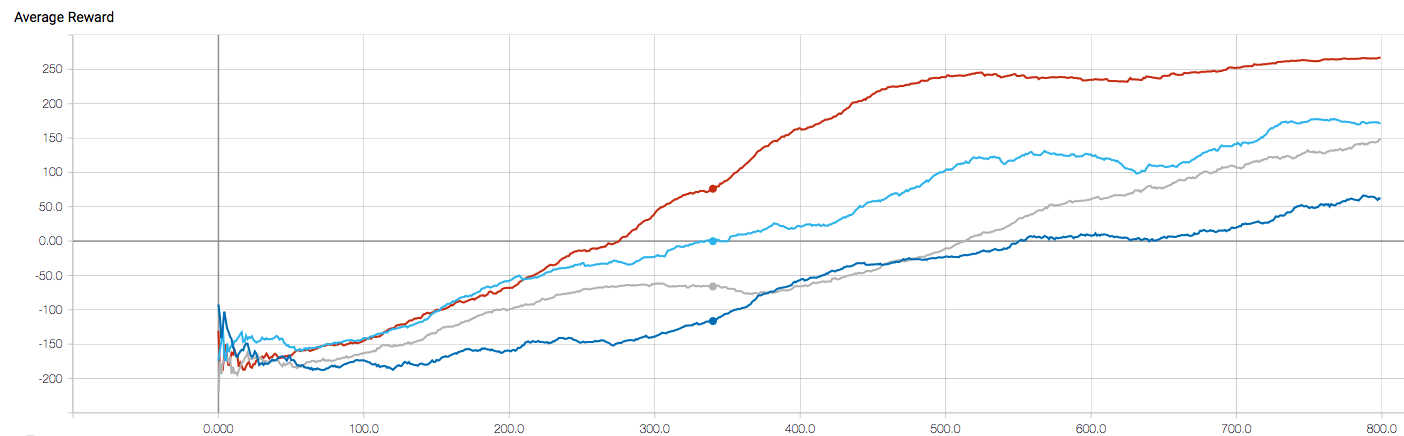
\includegraphics[scale=0.75,width=0.75\columnwidth]{figures/Hyperparameters1.png}%
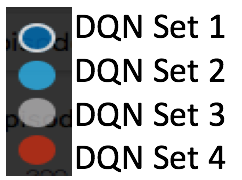
\includegraphics[scale=0.15,width=0.15\columnwidth]{figures/Hyperparameters_legends1.png}%
\caption{ Different Sets of hyperparamerts for DQN Model}%
\label{fig:HyperParameter Table}%
\end{figure}


\label{sec:exp1}
\begin{table}%
%\centering
\begin{tabular}{|l|c|c|c|c|c|}
\hline
Hyper-parameter & Set 1  & Set 2 & Set 3 & Set 4  \\
\hline
gamma & $0.99$ & $0.99$ & $0.99$ & $0.99$ \\
\hline
Epsilon(max,min,decay) & ($1$,$0$,$.998$) &  ($1$,$.01$,$.995$) &  ($1$,$.01$,$.998$) &  ($1$,$.01$,$.998$) \\
\hline
Learning Rate & $0.001$ & $0.0001$ & $0.0001$ & $0.0001$ \\
\hline
DNN layers & [$32$,$32$] &  [$128$,$32$] &  [$128$,$64$] &  [$128$,$64$] \\
\hline
Loss Function & MSE & MSE & MSE & MSE \\
\hline
Batch Size & $32$ & $32$  & $64$  & $64$  \\
\hline
Replay Memory Size & $2^{16}$ & $2^{16}$  & $2^{16}$  & $2^{16}$  \\
\hline
\end{tabular}
\caption{Different set of hyper-parameters were tried}
\label{tab:Hyper Parameter Set table}
\end{table}
%\vfill}
\subsection{ Error Analysis}
 After doing hyper-parameter tuning, our Agent was able to achieve average score of more than 200 quickly (at 435 episodes). 
However for some episodes after 435 the rewards were not consistently more than 200 for 100 iterations. This is due to the speed 
which is not getting reduced to zero (end state) although Lander is in landing zone.  The lunar lander is trying to bring itself to a zero velocity state and it tries to do so by applying thrust in opposite direction of landing horizontal velocity. In process of doing this, it applies alternate thrust from left and right side but is not able to bring the lander to complete halt to end the episode. Thus reducing the overall rewards and increases the number of frames. We observed that rewards are less than 200 when number of frames reaches the maximum value(1000). The Lunar Lander needs to learn how not to apply alternate left and right thrust to bring itself to a halt, taking no action will be the best action in this state. \\

Also, we observe the variation is more in DQN and Double DQN as compared to Dueling DQN. We got the best performance on Set 4 with Dueling DQN model.From figure 5, we can see that the agent underperforms about 4 \% of the time. Basically for these 4 cases, the game terminates because we have reached max frame count value (1000). This loss can be attributed to some unexplored states,


\begin{figure}[!ht]
%\begin{figure}%
%\vspace*{\fill}
\centering
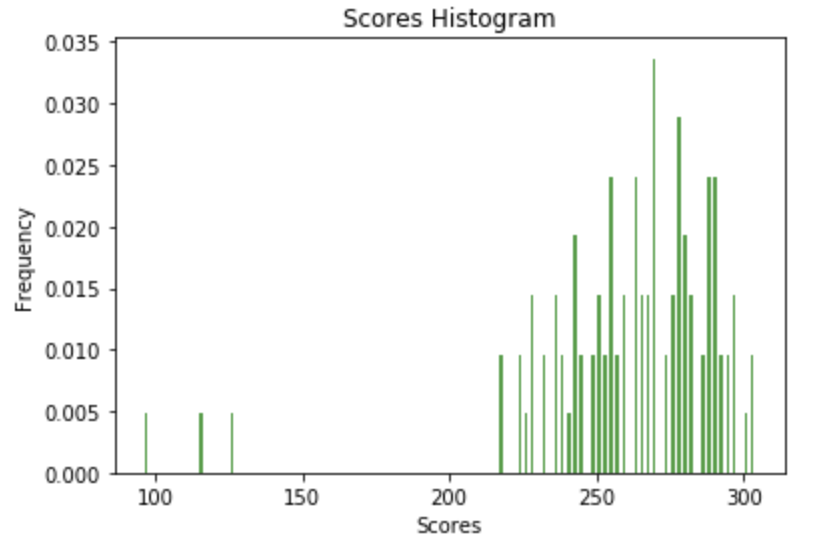
\includegraphics[scale=0.50,width=0.50\columnwidth]{figures/Histogram.png}%
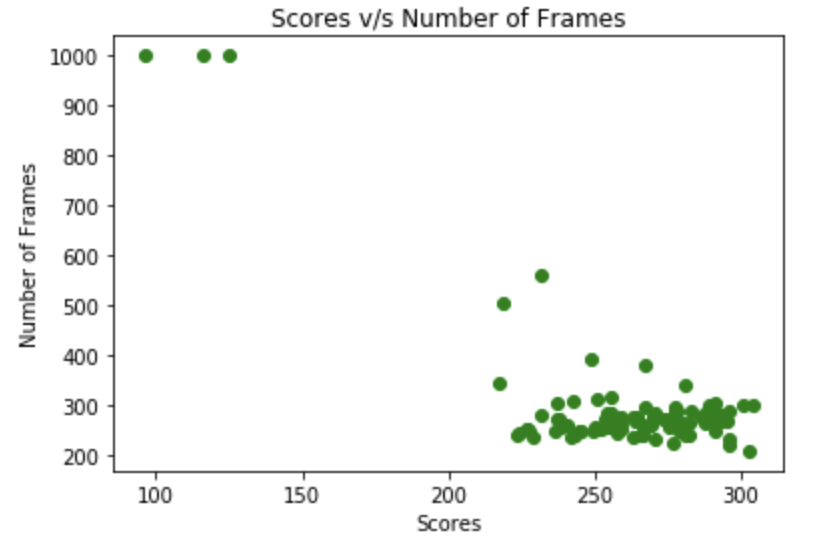
\includegraphics[scale=0.50,width=0.50\columnwidth]{figures/Frames.png}%
\caption{ Error Analysis : Distribution of scores for 100 episodes after the agent has learned }

\label{fig:Error Analysis}%
\end{figure}
%\vfill}

\subsection{ Comparision of DQN Variants}

Figure 6 shows comparison of different learning algorithms. The learning performance of baselines are also depicted in the same figure. From the figure, we can see that Dueling Network Architecture reaches the average reward 200 earlier than DQN and Double DQN, near episode number 450. \\

After reaching the reward 200, the graph is getting closer to zero slope. This is also intuitive since after reward 200, the average reward doesn’t change much. \\

Another thing evident from this is that the average reward for the random baseline fixes to a negative value after 600 episodes and there’s no much variation on average reward (although the reward for each episode varies significantly). \\
 
\begin{figure}[!ht]
%\begin{figure}%
%\vspace*{\fill}
\centering
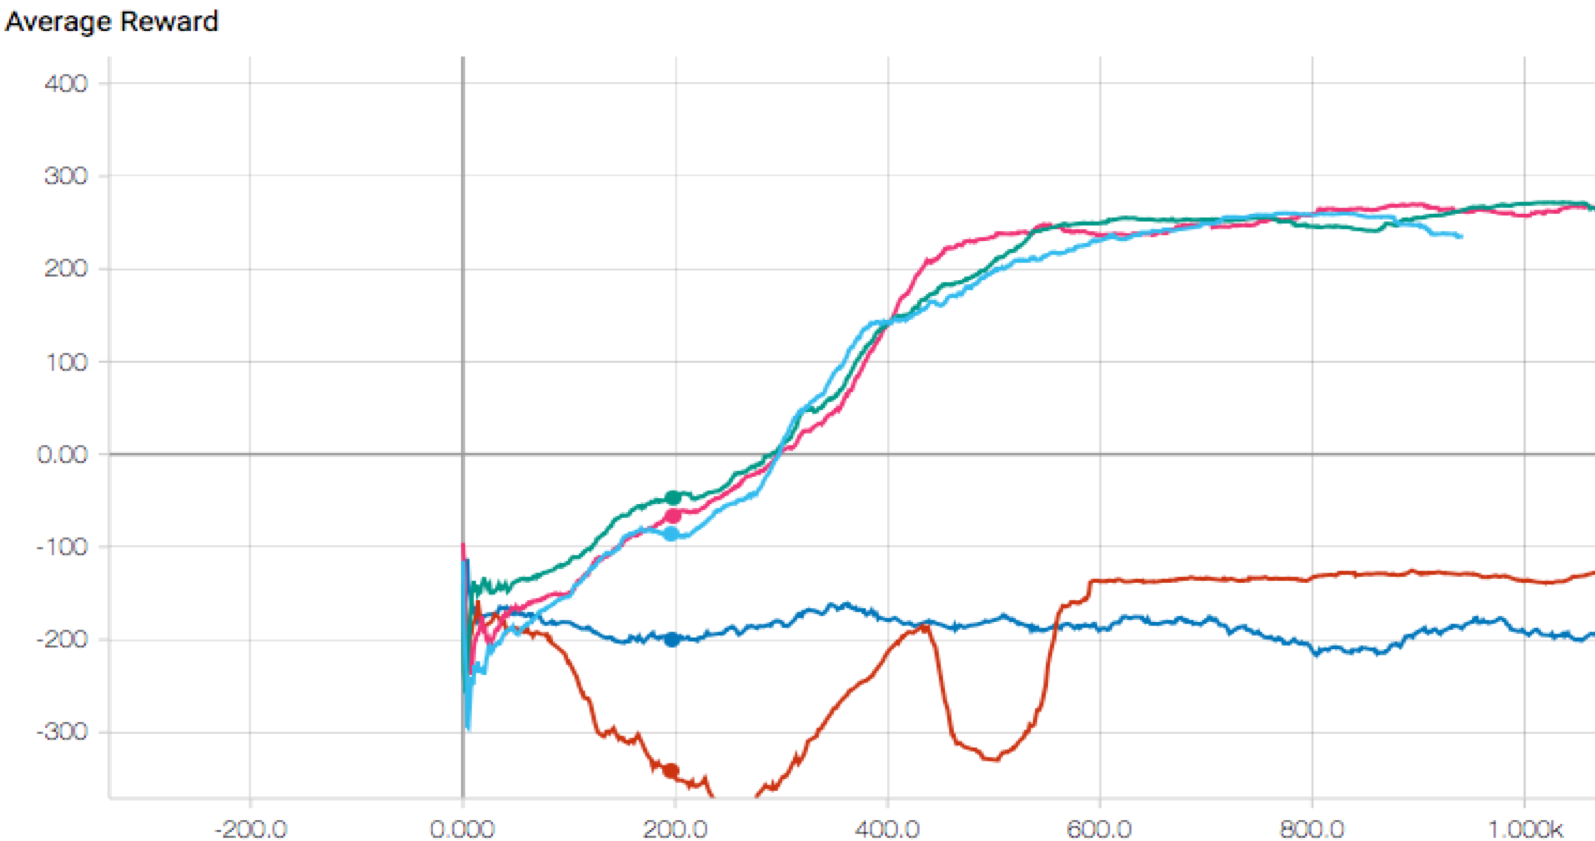
\includegraphics[scale=0.75,width=0.75\columnwidth]{figures/Picture1.png}%
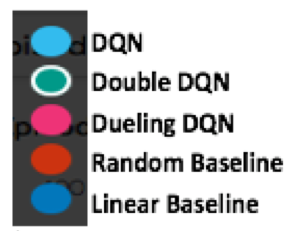
\includegraphics[scale=0.15,width=0.15\columnwidth]{figures/Legend.png}%
\caption{ Rewards for different approaches on tensor board}%
\label{fig:Visualization}%
\end{figure}
%\vfill}

\label{sec:exp}
\begin{table}%
\centering
\begin{tabular}{|l|c|c|}
\hline
Model & Avg. Score  & Number of episodes to reach 200 score  \\
\hline
Baseline & $-200$ & never \\
\hline
Linear Baseline & $-150$ & never \\
\hline
DQN & $123$ & $525$ \\
\hline
Double DQN & $220$ & $500$ \\
\hline
Dueling DQN & $225$ & $435$ \\
\hline
\end{tabular}
\caption{Comparision of Results for different model implementations}
\label{tab:Variants of DQN}
\end{table}


\subsection{ Model Evaluation}

All aforementioned models are evaluated for 100 episodes for a fixed weights as shown in Figure 7(left side). \\  
\begin{figure}[!ht]
%\begin{figure}%
%\vspace*{\fill}
\centering
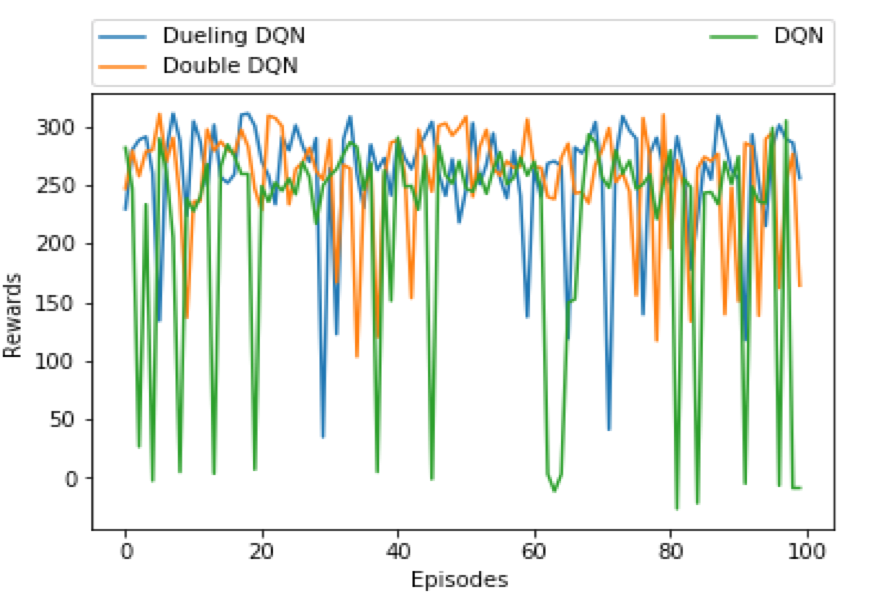
\includegraphics[scale=0.50,width=0.50\columnwidth]{figures/Picture2.png}%
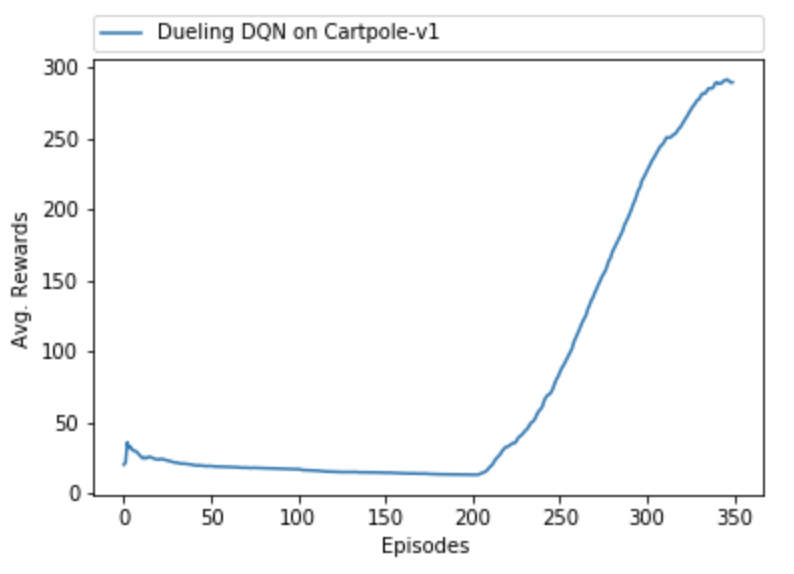
\includegraphics[scale=0.50,width=0.50\columnwidth]{figures/Cartpolev1.png}%
%\caption{ Agent learning CartPole Game}%

\caption{ Evaluating Performance of different DQN Networks and Agent learning CartPole-v1 Game}%
\label{fig:Different DQN Performance}%
\end{figure}
%\vfill}

\subsection{ Agent on other Environments}
We used the Agent to train on "CartPole-v1" game environment and were able to achieve good results. After Our AI agent successfully learnt the game as shown in Figure 7(right side) and consecutively won it. This proves the generality of the algorithm.


\section{Conclusion}
\label{sec:conclusion}

The project successfully completes the original scope, having produced a working reinforcement learning agent and providing a study and comparison of variants of DQN. DQN was applied effectively on this specific problem, and produced successful results. The success strengthens the use and generality of this algorithm on other problems. (FIXME add  cartpole)

An agent with too high of a discount was unable to credit actions to success, far enough in the future. Simply put, it was too myopic. As a result, agents learned how to hover, but never learned how to land. We also observed effect of having smaller replay-memory size. Sometimes a drop in the rewards after model learns is because after many consecutive successes, the replay buffer won't have many failure cases to train on. So, it used to 'forget' how to recover from many failure cases.

The DQN variants we tried gave very good results once the hyperparameters were tuned correctly. When implemented the algorithm code in a modularized format, we could easily change the parameters and play with it. Also, minimal tweaks were required for each the DQN variant. Not much of hyperparameter tuning was required across DQN variants. Given more time and resources, the agent could have been tuned via a more exhaustive grid search. After some literature review, we thought DQN could also have been enhanced with prioritized replay however, we did not observe any improvement. Rather the learning time was about 1000 episodes(FIXME). Lastly, the more advanced Duel Q-learning learner undoubtedly increased the accuracy of the reinforcement learning agent. 
\section{Codalab Link}
\label{sec:conclusion}

https://worksheets.codalab.org/worksheets/0x1e3fc24cfa0d4ff3b492d0f47b6e0887/
 \\
command to run \\

cl run :brain.py :hyperparameters.py :main.py :agent.py :environment.py :memory.py initial_weights:0xc8fff4 'python3 main.py --should_learn=False --agent=Dueling --initial_weights=initial_weights' -n sort-run --request-docker-image prabhjotrai/openai-gym:v1 \\
FIX ME Verify this once  \\
%\pagestyle{plain}

\bibliography{biblio}
\bibliographystyle{abbrv}
%\newpage
%%\section{Contributions}
\label{contributions}
All of us contributed in the discussions about what problem to target,  and what techniques to apply.
All of us helped with writing and reviewing the report.


\section{Appendix}
\subsection{Implementation choices}

The choice of state was based on the actual configuration of the lunar lander, and we learnt weights for each feature in the state. Another choice could have been training on image data, feeding images per episode and learning on gained rewards. Since this would have been computationally expensive, we chose the former approach to explicit definition of state space and learning it's weights. \\

For running different algorithms, we created separate classes so that the code is not only modularized, but can also be run easily on different openai environments, learning algorithms can be easily changed etc. Here's a quick description of different classes:

\begin{enumerate}
\item \textbf{Brain:} Class which contains keras models, updates the weights through train function and performs prediction based on learnt weights. 
\item \textbf{Memory:} Class which appends observations until maximum memory length and samples based on given batch size hyperparameter
\item \textbf{Agent:} Our agent class which explores and exploits based on fixed hyperparameters(gamma, epsilon max, epsilon min and decay) and passed arguments. This is also the class where we are performing the replay action and training the agent's brain instance. It also contains another instance of memory class which is used in replay while sampling.
\item \textbf{Environment:} Class which runs the episode on given agent and asks the agent to observe and replay whenever the agent is trying to learn on episodes. It returns the information on how much reward was observed on each episode and for how long each episode ran
\end{enumerate}

\end{document}

